% WEB APPLICATION
\subsubsection{Web Application}
\vspace{-2em}
\begin{figure}[H]
    \centering
    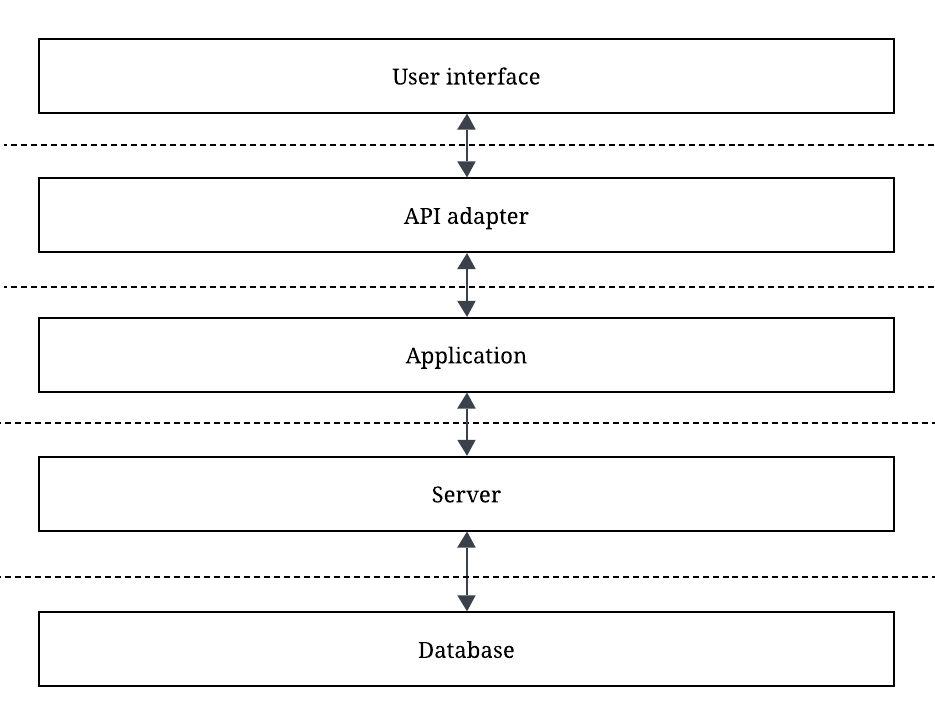
\includegraphics[width=1\textwidth]{images/bld_web_application.png}
    \vspace{-2em}
    \caption{Block Diagram of the Web application.}
    \label{fig:block_diagram_web}
\end{figure}
\begin{minipage}{\textwidth}
    \setlength{\parindent}{2em}
    \textbf{\autoref{fig:block_diagram_web}} above illustrates the high-level block diagram of the GMES School \textbf{web application system}. The architecture follows a layered approach where users interact with the system through the \textbf{User Interface} layer at the top. User requests are channeled through the \textbf{API Adapter}, which serves as the communication bridge between the frontend and backend services. These requests are processed by core services in the \textbf{Application layer}, which contains the business logic and application-specific functionality. The \textbf{Server layer} provides the runtime environment and infrastructure support, managing system resources, HTTP protocols, STOMP protocols, and service deployment. Finally, all processed data is stored and retrieved from the \textbf{Database layer}, which ensures data persistence, integrity, and security across the entire system.
\end{minipage}\\

\setlength{\parindent}{2em}Additionally, the system implements role-based access control, so that the application layer will provide different services and features based on the user's role.
% EMPLOYEE
\vspace{-0.4cm}
\begin{figure}[H]
    \centering
    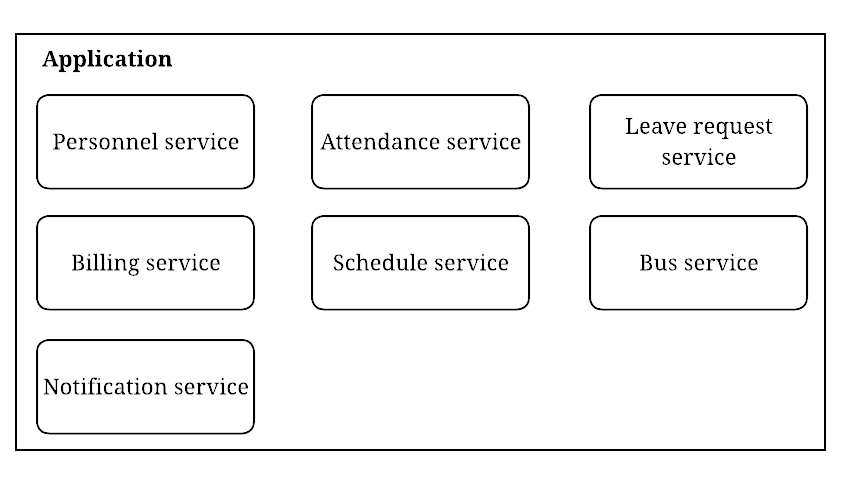
\includegraphics[width=0.8\textwidth]{images/bld_employee_web.png}
    \vspace{-1em}
    \caption{Application layer of the Web application for employees.}
    \label{fig:block_diagram_employee_web}
\end{figure}
\vspace{-0.4cm}
\setlength{\parindent}{2em} For \textbf{employees} (teachers and staff), the system provides several services illustrated in \textbf{\autoref{fig:block_diagram_employee_web}} that allow them to manage personnel records, attendance tracking, leave requests, salary processing, fee, scheduling, bus transportation, and notification.

% ADMIN
\vspace{-0.4cm}
\begin{figure}[H]
    \centering
    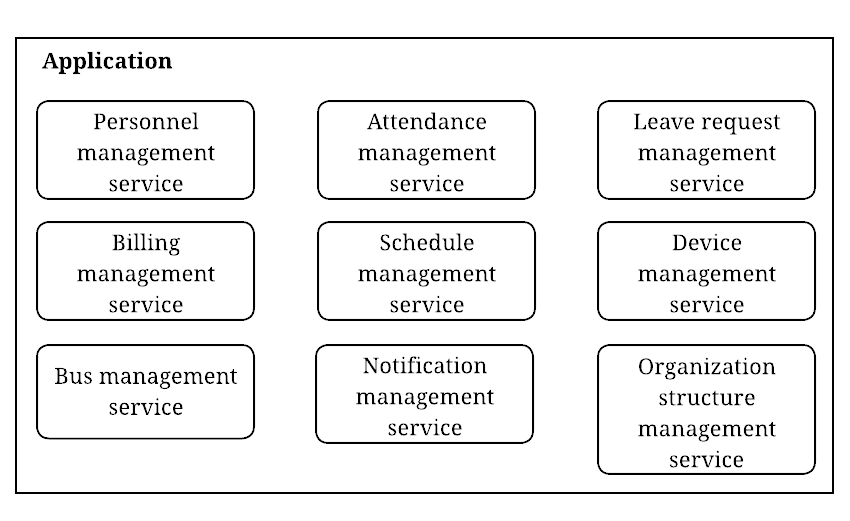
\includegraphics[width=0.8\textwidth]{images/bld_admin_web.png}
    \vspace{-1em}
    \caption{Application layer of the Web application for administrators.}
    \label{fig:block_diagram_admin_web}
\end{figure}
\vspace{-0.4cm}
\setlength{\parindent}{2em} For \textbf{administrators}, they have full access to all services that illustrated in \textbf{\autoref{fig:block_diagram_admin_web}}, complete oversight and control over all school operations through a unified platform.

% \setlength{\parindent}{2em}However, the functionality of these services will be hidden or provided based on the user's type and assigned role. This ensures that employees only access features relevant to their responsibilities and authorization level.


%MOBILE APP
\subsubsection{Mobile Application}
\begin{minipage}{\textwidth}
    \setlength{\parindent}{2em}
    The mobile application's architecture follows the same layered approach as the web application, as illustrated in \textbf{\autoref{fig:block_diagram_web}}.
\end{minipage}\\[0.17cm]
\indent Currently, the system's mobile application supports only three types of users: parents, teachers, and transportation staff. Therefore, the application layer provides different services and features based on the user type.
%TEACHER
\vspace{-0.7cm}
\begin{figure}[H]
    \centering
    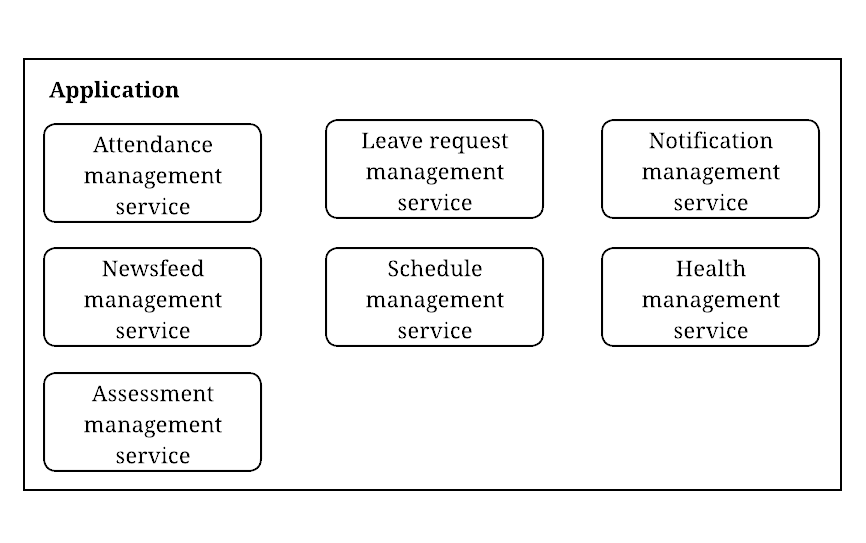
\includegraphics[width=0.8\textwidth]{images/bld_teacher_mobile_app.png}
    \vspace{-2em}
    \caption{Application layer of the Mobile Application for teachers.}
    \label{fig:block_diagram_teacher_mobile_app}
\end{figure}
\vspace{-0.4cm}
\setlength{\parindent}{2em}For \textbf{teachers}, the application layer integrates seven core services, as illustrated in \textbf{\autoref{fig:block_diagram_teacher_mobile_app}}, covering attendance, leave request, notifications, newsfeed, scheduling, health, and assessments. These integration services eliminate manual paperwork and time-consuming processes, help efficiently manage student-related activities, and maintain better communication with parents.
% PARENT MOBILE
\vspace{-0.7cm}
\begin{figure}[H]
    \centering
    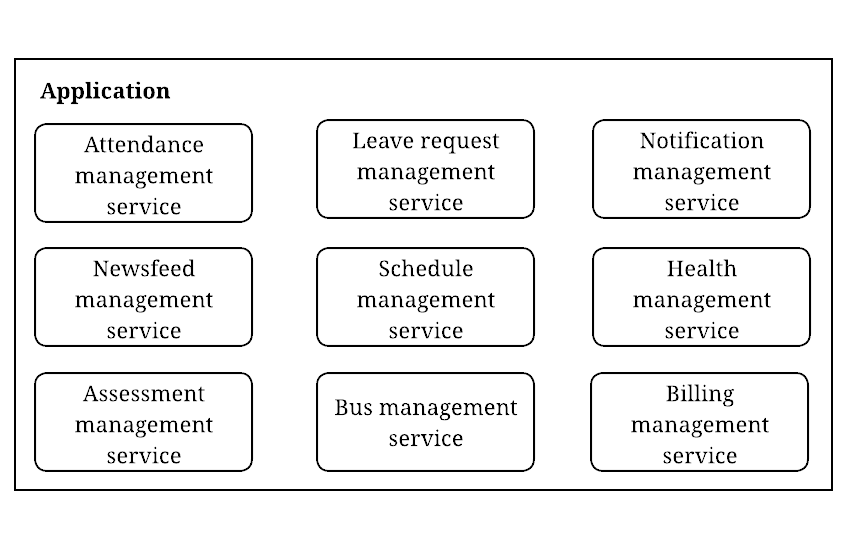
\includegraphics[width=0.8\textwidth]{images/bld_parent_mobile_app.png}
    \vspace{-2em}
    \caption{Application layer of the Mobile Application for parent.}
    \label{fig:block_diagram_parent_mobile_app}
\end{figure}
\vspace{-0.4cm}
\setlength{\parindent}{2em}For \textbf{parents}, the application layer provides several services, as illustrated in \textbf{\autoref{fig:block_diagram_parent_mobile_app}} that allow them to manage all aspects related to their children at school. By integrating these services into a single, user-friendly application, parents can gain greater control and convenience in supporting their children’s education.

% BUS MANAGER MOBILE APP
\begin{figure}[H]
    \centering
    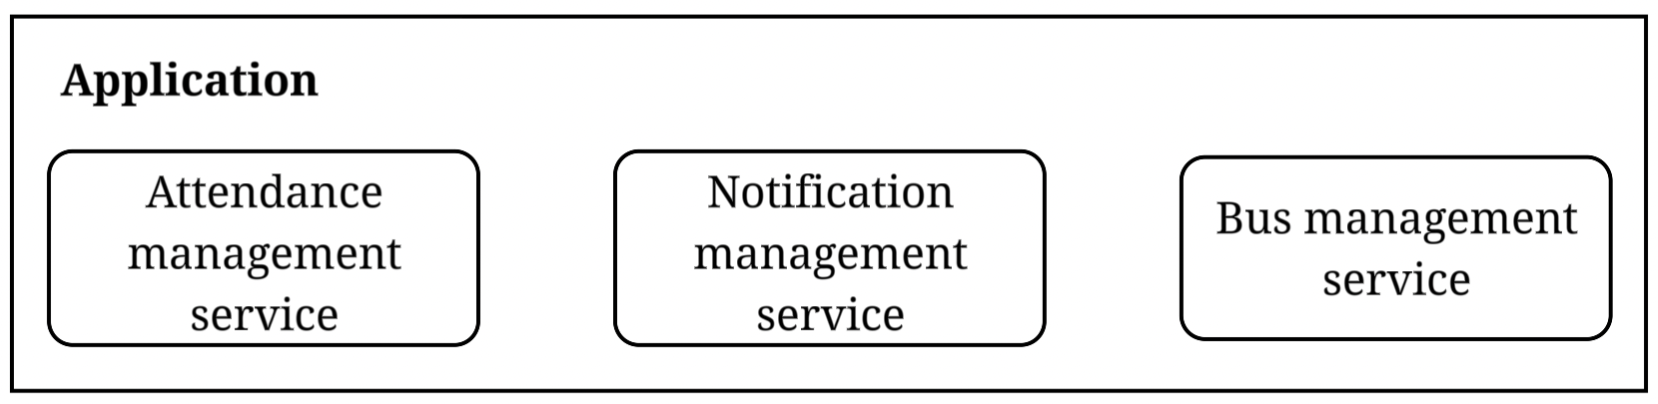
\includegraphics[width=0.8\textwidth]{images/bld_bus_manager_mobile_app.png}
    \vspace{-0.2em}
    \caption{Application layer of the Mobile Application for transportation staff.}
    \label{fig:block_diagram_bus_manager_mobile_app}
\end{figure}
\vspace{-0.4cm}
\setlength{\parindent}{2em}For \textbf{transportation staff}, the application provides only three services, as illustrated in \textbf{\autoref{fig:block_diagram_bus_manager_mobile_app}}. These services enable bus managers to efficiently manage bus routes, notifications and monitor student attendance during transportation.